\documentclass[10pt]{article}

\usepackage{graphicx} \usepackage{amssymb} \usepackage{amsmath}
\usepackage{amsfonts} \usepackage{verbatim} \usepackage{indentfirst}
\usepackage{amsthm} \usepackage{framed} \usepackage{quoted}
\usepackage{cite}


\usepackage[normalem]{ulem}

\usepackage{setspace}
%%%%%
% Setup
%%%%%

% Margins
\setlength{\textwidth}{5.5in} \setlength{\oddsidemargin}{0.5in}
\setlength{\evensidemargin}{0.5in}

\setlength{\textheight}{8.5in} \setlength{\topmargin}{0in}

% Conversations
\newcounter{convnum} \newenvironment{conversation} {\begin{framed}
\noindent{\textsc{Conversation
    \arabic{convnum}\addtocounter{convnum}{1}}}
\begin{description}
} {\end{description}
\end{framed}}

\newcommand{\machine}{\item[Machine:]}

\newcommand{\user}{\item[User:]}

% Theorem setup
\newtheorem{mythm}{Theorem} \newtheorem{mylem}{Lemma}
\newtheorem{mycor}{Corollary} \newtheorem{myex}{Example}

\def\squarebox#1{\hbox to #1{\hfill\vbox to #1{\vfill}}}
\newcommand{\qedbox}
           {\vbox{\hrule\hbox{\vrule\squarebox{.667em}\vrule}\hrule}}

\title{Automated Elementary Geometry Theorem Discovery via Inductive
  Diagram Manipulation\\ {\large MIT EECS MEng Thesis Proposal}}
\author{Lars Johnson (larsj@mit.edu)} \date{January 2015}

%%%%%
% Document
%%%%%
\begin{document}
\pagestyle{myheadings} \maketitle
% \onehalfspacing
\onehalfspacing \markright{MEng Thesis Proposal - Lars Johnson}
\section{Overview}
Understanding elementary geometry is a fundamental reasoning skill,
and encompasses a domain both constrained enough to model effectively,
yet rich enough to allow for interesting insights.  Although
elementary geometry knowledge can be conveyed via series of factual
definitions, theorems, and proofs, a particularly intriguing aspect of
geometry is the ability for students to learn and develop an
understanding of core concepts through visual investigation,
exploration, and discovery.

These visual reasoning skills reflect many of the cognitive activities
used as one interacts with his or her surroundings.  Day-to-day
decisions regularly rely on visual reasoning processes such as
imagining what three dimensional objects look like from other angles,
or mentally simulating the effects of one's actions on objects based
on a learned understanding of physics and the object's properties.
Such skills and inferred rules are developed through repeated
observation, followed by the formation and evaluation of conjectures.

Similar to such day-to-day three-dimensional reasoning, visualizing
and manipulating 2D geometric diagrams ``in the mind's eye'' allows
one to explore questions such as ``what happens if...''  or ``is it
always true that...''  to discover new conjectures.  Further
investigation of examples can increase one's belief in such a
conjecture, and an accompanying system of deductive reasoning from
basic axioms could prove that an observation is correct.

As an example, a curious student might notice that in a certain
drawing of a triangle, the three perpendicular bisectors of the edges
are concurrent, and that a circle constructed with center at the point
of concurrence intersects all three vertices of the triangle.  Given
this ``interesting observation,'' the student might explore other
triangles to see if this behavior is just coincidence, or conjecture
about whether it applies to certain classes of triangles or all
triangles in general.  After investigating several other examples, the
student might have sufficient belief in the conjecture to explore
using previously-proven theorems (in this case, correspondences in
congruent triangles) to prove the conjecture.  My proposed project is
a software system that simulates and automates this inductive thought
process.

\newpage
Automating geometric reasoning is not new, and has been an active
field in computing and artificial intelligence.  Dynamic geometry
software, automated proof assistants, deductive databases, and several
reformulations into abstract algebra models have been proposed in the
last few decades.  Although many of these projects have focused on the
end goal of obtaining rigorous proofs of geometric theorems, I am
particularly interested in exploring and modeling the more creative
human-like thought processes of inductively exploring and manipulating
diagrams to \emph{discover} new insights about geometry.

I propose the creation and analysis of an interactive computer system
that emulates the curious student described above, and is capable of
exploring geometric concepts through inductive investigation.  The
system will begin with a fairly limited set of factual knowledge
regarding basic definitions in geometry and provide means by which a
user interacting with the system could ``teach'' the system additional
geometric concepts and theorems by suggesting investigations the
system should explore to see if it ``notices anything interesting.''

To evaluate its recognition of such concepts, the interactive system
will provide means for a user to extract the observations and apply
its findings to new scenarios.  In addition to the automated reasoning
and symbolic artificial intelligence aspects of a system that can
learn and reason inductively about geometry, the project also has some
interesting opportunities to explore educational concepts related to
experiential learning, and several extensions to integrate it with
existing construction synthesis and proof systems.

\section{Manipulating  Diagrams ``In the Mind's Eye''}

Although the field of mathematics has developed a rigorous structure
of deductive proofs explaining most findings in geometry, much of
human intuition and initial reasoning about geometric ideas come not
from applying formal rules, but rather from visually manipulating
diagrams ``in the mind's eye.''

\singlespacing
\subsection{An Initial Example}

\begin{center}
\includegraphics[width=0.90\textwidth]{diagrams/rectangles.eps}
\end{center}

\noindent {\bf Example 1: Of the three diagrams above, determine which
  have constraints sufficient to restrict the quadrilateral $ABCD$ to
  always be a rectangle.}

\onehalfspacing

An automated deductive solution to this question could attempt to use
forward-chaining of known theorems to determine whether there was a
logical path that led from the given constraints to the desired result
that the quadrilateral shown is a rectangle.  However, getting the
correct results would require having a rich enough set of inference
rules and a valid system of applying them.

\newpage
A more intuitive visual-reasoning approach usually first explored by
humans is to initially verify that the marked constraints hold for the
instance of the diagram as drawn and then mentally manipulate or
``wiggle'' the diagram to see if one can find a nearby counter-example
that still satisfies the given constraints, but is not a rectangle.
If the viewer is unable to find a counter-example after several
attempts, he or she may be sufficiently convinced the conclusion is
true, and could commit to exploring a more rigorous deductive proof.

\singlespacing

\begin{center}
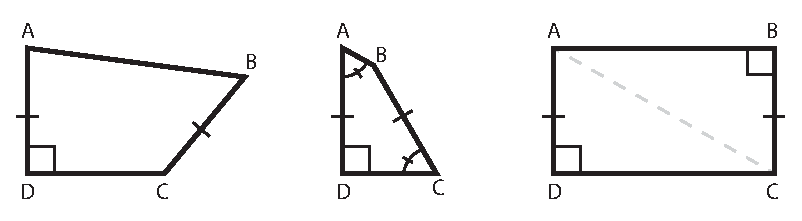
\includegraphics[width=0.80\textwidth]{diagrams/rectangles-answer.eps}
\end{center}

\noindent {\bf Solution to Example 1: As the reader likely discovered,
  the first two diagrams can be manipulated to yield instances that
  are not rectangles, while the third is sufficiently constrained to
  always represent a rectangle.  (This can be proved by adding a
  diagonal and using the Pythagorean theorem.)}

\onehalfspacing

\subsection{Diagrams, Figures, and Constraints}

This example of manipulation using the ``mind's eye'' also introduces
some terminology helpful in discussing the differences between images
as drawn and the spaces of geometric objects they represent.  For
clarity, a \emph{figure} will refer to an actual configuration of
points, lines, and circles drawn on a page.  Constraint annotations
(congruence or measure) added to a figure create a \emph{diagram},
which represents the entire space of figure \emph{instances} that
satisfy the constraints.

An annotated figure presented on a page is typically an instance of
its corresponding diagram.  However, it is certainly possible to add
annotations to a figure that are not satisfied by that figure,
yielding impossible diagrams.  In such a case the diagram represents
an empty set of satisfying figures.

In the initial example above, the three quadrilaterals figures are
drawn as rectangles.  It is true that all quadrilateral figures in the
space represented by the third diagram are rectangles.  However, the
space of quadrilaterals represented by the first two diagrams include
instances that are not rectangles, as shown above.  At this time, we
will only start with valid diagrams whose constraints are satisfied in
the given figure.  However, detecting and explaining inconsistent
diagrams could be an interesting extension.

\section{Geometry Investigation}

These same ``mind's eye'' reasoning techniques can be used to discover
and learn new geometric theorems.  Given some ``interesting
properties'' in a particular figure, one can construct other instances
of the diagram to examine if the properties appear to hold uniformly,
or if they were just coincidences in the initial drawing.  Properties
that are satisfied repeatedly can be further explored and proved using
deductive reasoning.  The examples below provide several
demonstrations of such inductive investigations.

\subsection{Vertical Angles}

\singlespacing

\begin{center}
\includegraphics[width=0.9\textwidth]{diagrams/vertical.eps}
\end{center}

\noindent {\bf Investigation 1: Construct a pair of vertical angles.
  Notice anything interesting?}

\onehalfspacing

Often one of the first theorems in a geometry course, the fact that
vertical angles are equal is one of the simplest examples of applying
``mind's eye'' visual reasoning.  Given the diagram on the left, one
could ``wiggle'' the two lines in his or her mind and imagine how the
angles respond.  In doing so, one would notice that the lower angle's
measure increases and decreases proportionately with that of the top
angle.  This mental simulation, perhaps accompanied by a few drawn and
measured figures, could sufficiently convince the viewer that vertical
angles always have equal measure.

Of course, this fact can also be proved deductively by adding up pairs
of angles that sum to 180 degrees.  However, the inductive
manipulations are more reflective of the initial, intuitive process
one typically takes when first presented with understanding a diagram.

\singlespacing

\subsection{Elementary Results}
\label{sec:elem}

\begin{center}
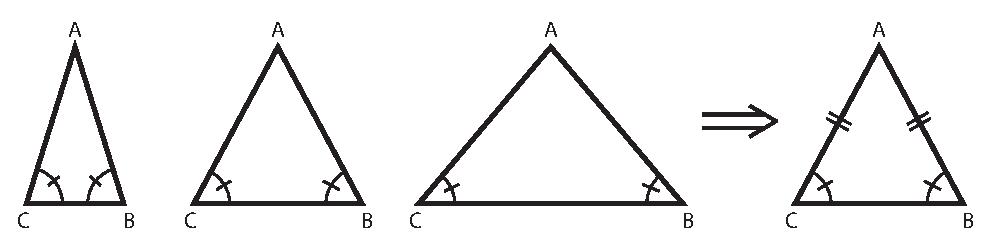
\includegraphics[width=0.9\textwidth]{diagrams/isoceles-triangle.eps}
\end{center}

\noindent {\bf Investigation 2: Construct a triangle $ABC$ with
  $\angle B = \angle C$.  Notice anything interesting?}

\onehalfspacing

A slightly more involved example includes discovering that if a
triangle has two congruent angles, it is isoceles.  As above, this
fact has a more rigorous proof that involves dropping an altitude from
point $A$ and using corresponding parts of congruent triangles to
demonstrate the equality of $AB$ and $AC$.  However, the inductive
investigation of figures that satisfy the constraints can yield the
same conjecture, give students better intuition for what is happening,
and help guide the discovery and assembly of known rules to be applied
in future situations.

In this and further examples, an important question becomes what
properties are considered ``interesting'' and worth investigating in
further instances of the diagram, as discussed in section
\ref{sec:interest}.  As suggested by the examples in Investigation 3,
this can include relations between segment and angle lengths,
concurrent lines, collinear points, or parallel and perpendicular
lines.

\singlespacing

\begin{center}
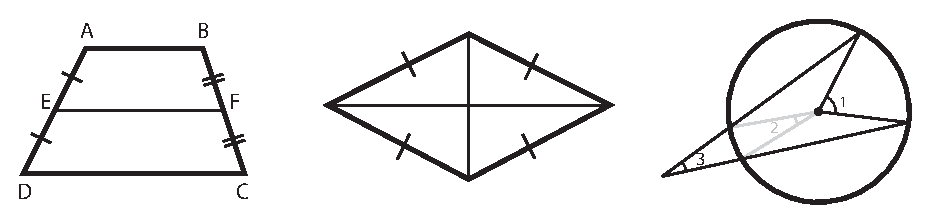
\includegraphics[width=0.95\textwidth]{diagrams/extra-diagrams.eps}
\end{center}

\noindent {\bf Investigation 3: What is interesting about the
  relationship between $AB$, $CD$, and $EF$ in the trapezoid? What is
  interesting about the diagonals of a rhombus? What is interesting
  about $\angle 1$, $\angle 2$, and $\angle 3$?}

\onehalfspacing


\subsection{Nine Point Circle and Euler Segment}

Finally, this technique can be used to explore and discover
conjectures well beyond the scope of what one can visualize in his or
her head:

\singlespacing

\begin{center}
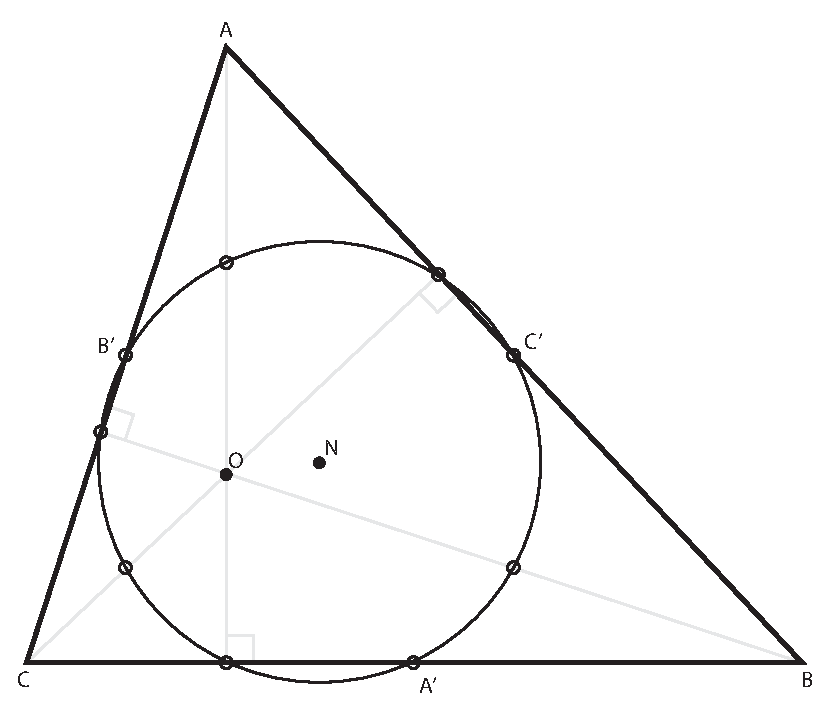
\includegraphics[width=0.6\textwidth]{diagrams/nine-point.eps}
\end{center}

\noindent {\bf Investigation 4a: In triangle $ABC$, construct the side
  midpoints $A'$, $B'$, $C'$, and orthocenter $O$ (from altitudes).
  Then, construct the midpoints of the segments connecting the
  orthocenter with each triangle vertex.  Notice anything
  interesting?}

\onehalfspacing

As a more complicated example, consider the extended investigation of
the Nine Point Circle and Euler Segment.  As shown in Investigation
4a, the nine points created (feet of the altitudes, midpoints of
sides, and midpoints of segments from orthocenter to vertices) are all
concentric, lying on a circle with center labeled $N$.

Upon first constructing this figure, this fact seems almost beyond
chance.  However, as shown in Investigation 4b (below), further
``interesting properties'' continue to appear as one constructs the
centroid and circumcenter: All four of these special points ($O$, $N$,
$D$, and $M$) are collinear on what is called the \emph{Euler
  Segment}, and the ratios $ON:ND:DM$ of $3:1:2$ hold for any
triangle.

\singlespacing

\begin{center}
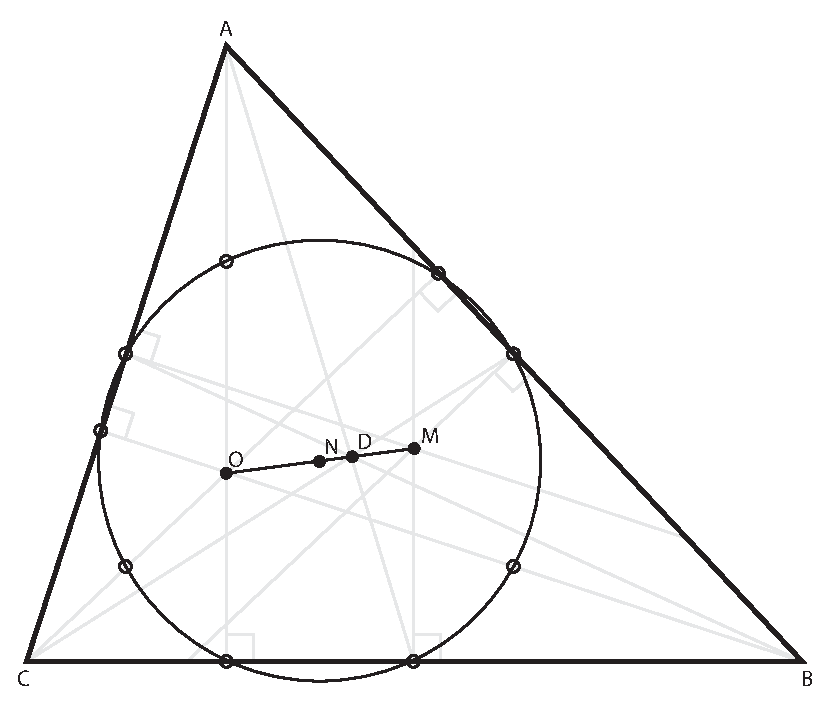
\includegraphics[width=0.7\textwidth]{diagrams/euler-line.eps}
\end{center}

\noindent {\bf Investigation 4b: Continue the investigation from 4a by
  also constructing the centroid $D$ (from medians) and circumcenter
  $M$ (from perpendicular bisectors).  Notice anything interesting?  }

\onehalfspacing
\section{Proposed Software Implementation}

My proposed MEng project involves building and analyzing a software
implementation that can make such inductive observations and
discoveries as described above.  Although there are many aspects
involved in replicating the human-like reasoning discussed, I will
initially focus on a core system that is able to model the inductive
exploratory behavior.  Further abilities can be added as extensions or
applications of the core system as described in section
\ref{sec:extension}.

This core system will provide an interpreter to accept input of
construction instructions, an analytic geometry system that can create
instances of such constructions, a pattern-finding process to discover
``interesting properties'', and an interface for reporting findings.

\subsection{Interpreting Construction Steps}

The first step in such explorations is interpreting an input of the
diagram to be explored.  To avoid the problems involved with solving
constraint systems and the possibility of impossible diagrams, the
core system will take as input an explicit list of construction steps
that results in an instance of the desired diagram.  These
instructions can still include arbitrary selections (let $P$ be some
point on the line, or let $A$ be some acute angle), but otherwise will
be restricted to basic construction operations using a compass and
straight edge.

To simplify the input of more complicated diagrams, some of these
steps can be abstracted into a library of known construction
procedures.  For example, although the underlying figures will be
limited to very simple objects of points, lines, and angles, the steps
of constructing a triangle (three points and three segments) or
bisecting a line or angle can be encapsulated into single steps.

\subsection{Creating Figures}

Given a language for expressing the constructions, the second phase of
the system will be to perform such constructions to yield an instance
of the diagram.  This process will mimic ``imagining'' manipulations
and will result in an analytic representation of the figure with
coordinates for each point.  Arbitrary choices in the construction
(``Let $Q$ be some point not on the line.'') will be chosen via an
random process, but with an attempt to keep the figures within a
reasonable scale to ease human inspection.

\subsection{Noticing Interesting Properties}
\label{sec:interest}

Having constructed a particular figure, the system will need to be
able to examine it to find interesting properties.  These properties
involve facts that appear to be ``beyond coincidence''.  As mentioned
in section \ref{sec:elem}, this generally involves relationships
between measured values, but can also include ``unexpected''
configurations of points, lines, and circles.  As the system discovers
interesting properties, it will reconstruct the diagram using
difference choices and observe if the observed properties hold true
across many instances of a diagram.

\subsection{Reporting Findings}

Finally, once the system has discovered some interesting properties
that appear repeatedly in instances of a given diagram, it will need a
means of reporting its results to the user.  Although this could
easily be a simple list of all simple relationships, some effort will
be taken to avoid repeating observations that obvious in the
construction.  For example, if a perpendicular bisector of segment
$AB$ is requested, the fact that it bisects that segment in every
instance is not informative.  To do so, the construction process will
also maintain a list of facts that can be reasoned from construction
assumptions so that these can be omitted in the final reporting.

\section{Related Work}

The topics of automating geometric proofs and working with diagrams
are areas of active research.  Several examples of related work can be
found in the proceedings of annual conferences such as \emph{Automated
  Deduction in Geometry} \cite{autoDeduction} and \emph {Diagrammatic
  Representation and Inference} \cite{diagramInference}.  In addition,
two papers from the past year combine these concepts with a layer of
computer vision interpretation of diagrams.  Chen, Song, and Wang
present a system that infers what theorems are being illustrated from
images of diagrams \cite{fromImages}, and a paper by Seo and
Hajishirzi describes using textual descriptions of problems to improve
recognition of their accompanying figures \cite{diagramUnderstanding}.

Further related work includes descriptions of the educational impacts
of dynamic geometry approaches and some software to explore geometric
diagrams and proofs.  However, such software typically uses alternate
approaches to automate such processes, and few focus on inductive
reasoning.

\subsection{Dynamic Geometry}
From an education perspective, there are several texts that emphasize
an investigative, conjecture-based approach to teaching such as
\emph{Discovering Geometry} by Michael Serra \cite{serraDiscovering},
the text I used to learn geometry.  Some researchers praise these
investigative methods \cite{geoTransformations} while others question
whether it appropriately encourages deductive reasoning skills
\cite{geoTeaching}.

\subsection{Software}
Some of these teaching methods include accompanying software such as
Cabri Geometry \cite{cabri} and the Geometer's Sketchpad
\cite{geoSketchpad} designed to enable students to explore
constructions interactively.  These programs occasionally provide
scripting features, but have no proof-related automation.

A few more academic analogs of these programs introduce some proof
features.  For instance, GeoProof \cite{geoProof} integrates diagram
construction with verified proofs using a number of symbolic methods
carried out by the Coq Proof Assistant, and Geometry Explorer
\cite{geoExplorer} uses a full-angle method of chasing angle relations
to check assertions requested by the user.  However, none of the
software described simulates the exploratory, inductive investigation
process used by students first discovering new conjectures.

\subsection{Automated Proof and Discovery}
Although there are several papers that describe automated discovery or
proof in geometry, most of these use alternate, more algebraic methods
to prove theorems.  These approaches include an area method
\cite{autoTools}, Wu's Method involving systems of polynomial
equations \cite{wuMethod}, and a system based on Gr\"obner Bases
\cite{grobner}.  Some papers discuss reasoning systems including the
construction and application of a deductive database of geometric
theorems \cite{deductiveDatabase}.  However, all of these methods
focused either on deductive reasoning or complex algebraic
reformulations.

\section{Extensions and Applications}

\label{sec:extension}
There are several approaches that can extend the system and increase
its power.  These generally involve adding components before and after
the core elements to create a more complete geometry reasoning system.
Several of these components relate to existing work mentioned above
and can use such ideas as a basis for implementation. The diagram
demonstrates the connections between the core system and the
extensions described below.

\begin{center}
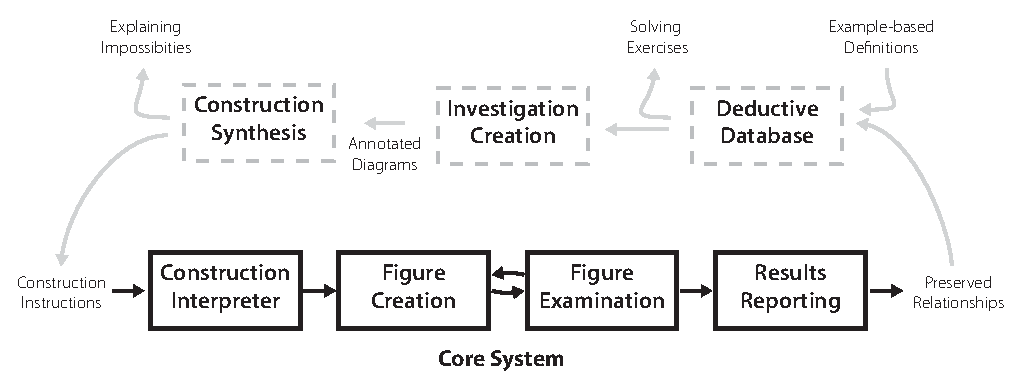
\includegraphics[width=\textwidth]{diagrams/system-diagram.eps}
\end{center}

\noindent {\bf System Diagram: Extensions of the core induction system
  could create a full loop and permit completely independent geometry
  investigation.}

\subsection{Deduction Databases and Proof Systems}

Making use of the findings of the core components, a deductive
automated proof system as discussed above could be used to prove or
verify newly discovered conjectures.  If proven, these theorems could
be stored in a deductive database and used as inference rules in
solving exercises.  This component would allow the system to
demonstrate and apply what it is learning to user-specified tasks and
exercises.

\subsection{Modeling Base Knowledge}

In addition to a deductive database of findings, the system could also
include a component in which it could learn new terminology and base
definitions.  For instance, rather than hard coding what it means for
a triangle to be isoceles, the system could allow a user to present
example and counterexample figures.  Based on patterns discovered in
these figures, the system could propose and test definitions to be
used in future investigations.  This dynamic base knowledge repository
could be used throughout the system.

\subsection{Construction Synthesis}

Preceding the input of the core system, a possible extension is to
synthesize construction instructions from an initial diagram.  Rather
than requiring explicit steps, the system thus could look at an
annotated diagram and derive a set of constructions that produces a
figure maintaining such constraints.  During this process, one would
also have to deal with impossible diagrams or complicated
constructions.  A recent paper by Microsoft Research discusses some of
these ideas \cite{synth}.

\subsection{Independent Investigation Creation}

Finally, if there is sufficient extension of a deductive library and
construction synthesis, an interesting extension would be one in which
the system proposes its own diagrams to investigate rather than being
prompted from an outside user.  This would provide some full circle
closure to the discovery process and could even lead to the system
creatively devising interesting exercises or exam questions that test
what it has acquired.

\section{Evaluation of System}

The experimentation and evaluation of the system will primarily
involve exploring what investigations it is able to pursue and what
conjectures it is able to discover.  Flexibility in implementation
will allow for the modification of base knowledge and characteristics
of what is ``interesting'' to see how these changes affect the
system's behavior and whether there is some sort of minimal assumed
knowledge that still enables the system to make interesting
discoveries.

\section{Conclusion}

Manipulating geometry diagrams in the ``mind’s eye'' reflects the
creative human process of discovery, and relates to the experiential
aspect of our “mind and hand” education.  Automating this reasoning
system can simulate some day to-day interactions and inferences,
allowing for an exploration of what can be learned using a more
inductive approach.  It will be exciting to explore these idea as I
continue to pursue my MEng project.

\bibliographystyle{IEEEtran} \bibliography{mybib}

\end{document}

%%  LocalWords:  Seo Hajishirzi Cabri GeoProof Coq Wu's Gr obner mybib
